\section{Cơ sở lý thuyết}

\subsection{Kho dữ liệu}

\subsubsection{Định nghĩa}
Kho dữ liệu (Data Warehouse - DW) không chỉ đơn thuần là một kho lưu trữ, mà là một hệ thống quản trị dữ liệu quy mô lớn, được thiết kế chuyên biệt để phục vụ cho công tác phân tích (Analytics) và hỗ trợ ra quyết định (Decision Support System - DSS). Theo định nghĩa kinh điển của Bill Inmon – người được mệnh danh là cha đẻ của kho dữ liệu, đây là một tập hợp dữ liệu hướng chủ đề, được tích hợp, có gắn mốc thời gian và mang tính phi biến động. 

Để hiểu rõ hơn, ta có thể so sánh kho dữ liệu với các cơ sở dữ liệu tác nghiệp thông thường (OLTP - Online Transaction Processing). Nếu OLTP được tối ưu hóa để xử lý hàng ngàn giao dịch ghi/xóa nhỏ lẻ, liên tục mỗi giây (ví dụ: hệ thống ghi nhận dữ liệu đo lường trực tiếp từ cảm biến IoT), thì kho dữ liệu lại thuộc hệ thống OLAP (Online Analytical Processing). Nó được tối ưu hóa cho các truy vấn đọc khối lượng lớn và phức tạp. Trong các bài toán học máy như dự đoán độ an toàn của nguồn nước, kho dữ liệu đóng vai trò là ``Nguồn sự thật duy nhất'' (Single Source of Truth), cung cấp nền tảng dữ liệu sạch, đáng tin cậy và đã qua xử lý để huấn luyện mô hình.

\subsubsection{Các đặc trưng của kho dữ liệu}
\begin{itemize}
    \item \textbf{Tính chủ đề (Subject-oriented):} Thay vì tổ chức dữ liệu theo từng chức năng của ứng dụng phần mềm (ví dụ: ứng dụng quản lý phòng thí nghiệm riêng, ứng dụng theo dõi trạm bơm riêng), kho dữ liệu tập trung xoay quanh các đối tượng nghiệp vụ cốt lõi. Trong ngữ cảnh của bài toán này, các chủ đề chính có thể là ``mẫu nước'', ``chỉ số hóa lý'', hay ``độ an toàn'' (Potability). Việc tập trung vào chủ đề giúp người phân tích hoặc kỹ sư dữ liệu dễ dàng khai thác thông tin đa chiều mà không cần quan tâm dữ liệu đó được sinh ra từ phần mềm gốc nào.
    
    \item \textbf{Tính tích hợp (Integrated):} Đây được xem là đặc trưng quan trọng nhất và tiêu tốn nhiều công sức nhất khi xây dựng kho dữ liệu. Dữ liệu đầu vào thường đến từ rất nhiều nguồn phân tán, đa dạng định dạng (file CSV từ phòng thí nghiệm, dữ liệu JSON từ API cảm biến, hoặc cơ sở dữ liệu SQL từ các trạm quan trắc cũ). Thông qua quá trình ETL (Extract - Transform - Load), toàn bộ dữ liệu sẽ được làm sạch, đồng nhất tên gọi, chuẩn hóa định dạng và quy đổi về cùng một hệ đơn vị đo lường (ví dụ: thống nhất chuẩn hóa đơn vị độ đục Turbidity, quy đổi nồng độ Sulfate hay Chloramines về cùng hệ đo). Khi nằm trong kho, dữ liệu rác hoặc dữ liệu mâu thuẫn đã bị loại bỏ để tạo thành một khối đồng nhất.
    
    \item \textbf{Tính thời gian (Time-variant):} Mỗi bản ghi trong kho dữ liệu đều gắn liền với một mốc hoặc một khoảng thời gian cụ thể. Khác với cơ sở dữ liệu thông thường chỉ lưu trữ trạng thái hiện tại (khi có dữ liệu mới thì ghi đè dữ liệu cũ), kho dữ liệu lưu trữ toàn bộ lịch sử biến động. Nhờ đó, ta có thể phân tích được xu hướng thay đổi chất lượng nguồn nước theo chu kỳ (ví dụ: so sánh độ cứng của nước giữa mùa mưa và mùa khô) hoặc theo dõi sự suy giảm chất lượng nước qua nhiều năm để đưa ra các dự báo dài hạn.
    
    \item \textbf{Tính phi biến động (Non-volatile):} Dữ liệu một khi đã được trích xuất, làm sạch và nạp vào kho thì sẽ đóng vai trò như một "cuốn biên niên sử" và gần như chỉ được dùng để đọc (read-only) phục vụ cho việc khai phá dữ liệu (Data Mining). Nó không bị xáo trộn, chỉnh sửa hay xóa bỏ bởi các thao tác cập nhật hằng ngày. Tính chất này mang ý nghĩa sống còn đối với việc xây dựng các mô hình học máy (như Support Vector Machine hay Random Forest), vì nó đảm bảo tính tái lập (reproducibility) – mô hình sẽ luôn được huấn luyện và đánh giá trên một bộ dữ liệu có tính nhất quán cao, không lo bị sai lệch kết quả do dữ liệu nền tảng bị thay đổi đột ngột.
\end{itemize}

\subsubsection{Kiến trúc của kho dữ liệu}
Kiến trúc của một kho dữ liệu tiêu chuẩn thường được thiết kế theo mô hình phân tầng (multi-tier architecture) nhằm tách biệt quá trình thu thập, xử lý và trình bày dữ liệu. Điều này giúp đảm bảo khả năng mở rộng, tính bảo mật và hiệu năng khi xử lý khối lượng dữ liệu lớn. Nhìn chung, kiến trúc này bao gồm 4 thành phần chính được minh họa ở Hình \ref{fig:dw-architecture}:

\begin{figure}[H]
    \centering
    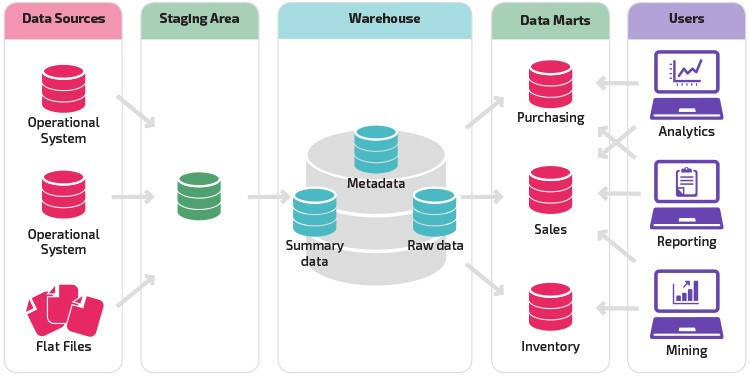
\includegraphics[width=0.8\linewidth]{IMAGE/DW-architecture.jpg}
    \caption{Kiến trúc của kho dữ liệu.}
    \label{fig:dw-architecture}
\end{figure}
\begin{enumerate}
    \item \textbf{Nguồn dữ liệu (Data Sources):} 
    Trong thực tế, dữ liệu hiếm khi nằm đồng nhất ở một nơi. Nguồn dữ liệu là lớp dưới cùng, nơi sản sinh hoặc chứa đựng dữ liệu gốc. Đối với hệ thống quản lý và phân tích chất lượng nước, dữ liệu có thể đến từ sự kết hợp của nhiều nguồn khác nhau:
    \begin{itemize}
        \item Các cơ sở dữ liệu quan hệ (RDBMS) của hệ thống quản lý trạm bơm hoặc phòng thí nghiệm (chứa thông tin mẫu thử, thời gian lấy mẫu).
        \item Dữ liệu từ các cảm biến IoT đo lường theo thời gian thực (được gọi qua các API API truyền tải dữ liệu JSON/XML về nhiệt độ, độ đục).
        \item Các tệp tin phẳng (Flat files) như CSV, Excel chứa dữ liệu ghi chép thủ công hoặc dữ liệu quan trắc lịch sử từ các cơ quan môi trường.
    \end{itemize}

    \item \textbf{Khu vực trung gian (Staging Area):} 
    Đây là vùng lưu trú tạm thời (landing zone) chuyên dùng để chứa dữ liệu thô vừa được trích xuất (Extract) từ các nguồn dữ liệu đa dạng kể trên. Mục đích chính của Staging Area là tạo ra một bộ đệm để thực hiện các tác vụ làm sạch và biến đổi dữ liệu (Transform) mà không gây áp lực tính toán lên các hệ thống nguồn OLTP đang vận hành. Tại đây, các kỹ sư dữ liệu sẽ thực hiện các thao tác quan trọng như:
    \begin{itemize}
        \item Xử lý các giá trị khuyết thiếu (Missing values), ví dụ như điền khuyết (imputation) cho các chỉ số pH hay Sulfate bị trống trong dữ liệu gốc.
        \item Loại bỏ các bản ghi trùng lặp và phát hiện các giá trị ngoại lai (Outliers) có thể làm sai lệch mô hình.
        \item Đồng nhất định dạng thời gian và quy đổi các đơn vị đo lường hóa lý về một chuẩn duy nhất.
    \end{itemize}

    \item \textbf{Kho lưu trữ trung tâm (Data Warehouse):} 
    Sau khi dữ liệu đã được làm sạch và chuẩn hóa hoàn toàn ở Staging Area, chúng sẽ được nạp (Load) vào kho lưu trữ trung tâm. Đây là trái tim của hệ thống, nơi lưu trữ toàn bộ dữ liệu lịch sử một cách có cấu trúc, tối ưu hóa cho các truy vấn phân tích phức tạp. Dữ liệu tại đây thường được mô hình hóa đa chiều (Dimensional Modeling) theo các lược đồ phổ biến:
    \begin{itemize}
        \item \textit{Star Schema (Lược đồ ngôi sao):} Cấu trúc phi chuẩn hóa, bao gồm một bảng Sự kiện trung tâm (Fact Table) lưu trữ các chỉ số định lượng (như nồng độ hóa chất, độ đục, độ cứng của nước) liên kết với các bảng Chiều (Dimension Tables) chứa thông tin mô tả (như thời gian, địa điểm, trạm quan trắc). Lược đồ này cho tốc độ truy vấn tương đối nhanh.
        \item \textit{Snowflake Schema (Lược đồ bông tuyết):} Là biến thể chuẩn hóa của Star Schema, trong đó các bảng Dimension được phân rã thành các bảng nhỏ hơn để tiết kiệm không gian lưu trữ, dù tốc độ truy vấn có thể chậm hơn đôi chút do phải kết nối (\texttt{JOIN}) nhiều bảng.
    \end{itemize}

    \item \textbf{Lớp trình bày dữ liệu (Information Delivery/Data Presentation):} 
    Đây là lớp giao tiếp cuối cùng, đóng vai trò phân phối dữ liệu từ kho lưu trữ trung tâm đến người dùng cuối hoặc các hệ thống nghiệp vụ khác. Tùy thuộc vào nhu cầu sử dụng, lớp này cung cấp các thành phần sau:
    \begin{itemize}
        \item \textbf{Data Mart:} Thay vì cho phép người dùng truy cập toàn bộ kho dữ liệu khổng lồ, Data Mart tạo ra các kho dữ liệu con, được trích xuất và tối ưu riêng cho từng nhóm đối tượng cụ thể. Ví dụ: một Data Mart chuyên biệt về 11Chỉ số an toàn nước'' dành riêng cho nhóm kỹ sư phát triển mô hình Machine Learning.
        \item \textbf{Công cụ phân tích và Trực quan hóa (BI Tools):} Kết nối với các nền tảng Business Intelligence (như Power BI, Tableau) để tạo ra các \textit{dashboard} theo dõi chất lượng nước theo thời gian thực.
        \item \textbf{Hệ thống Machine Learning:} Lớp này cung cấp nguồn dữ liệu đầu vào (đã được dán nhãn, làm sạch và tổng hợp) có độ tin cậy cao nhất để huấn luyện các thuật toán học máy như Support Vector Machine (SVM) hay Random Forest, từ đó dự đoán độ an toàn (Potability) của các mẫu nước mới trong tương lai.
    \end{itemize}
\end{enumerate}


\newpage

\subsection{Một số khái niệm khác}

\subsubsection{Quy trình ETL trong kho dữ liệu}
Quy trình ETL (Extract - Transform - Load) đóng vai trò cốt lõi trong kiến trúc của mọi hệ thống kho dữ liệu. Đặc biệt đối với các dự án ứng dụng học máy, chất lượng dữ liệu đầu vào là yếu tố quyết định trực tiếp đến độ chính xác của mô hình theo nguyên lý ``Garbage in, garbage out'' (Dữ liệu đầu vào kém sẽ tạo ra kết quả sai lệch). Do đó, ETL đảm nhiệm nhiệm vụ thiết yếu: sàng lọc, làm sạch và chuẩn hóa dữ liệu thô, từ đó kiến tạo một nền tảng dữ liệu đáng tin cậy trước khi bước vào giai đoạn phân tích chuyên sâu. Quy trình này được chia thành 3 giai đoạn chính:

\begin{itemize}
    \item \textbf{Extract (Trích xuất dữ liệu):} 
    Đây là bước thu thập dữ liệu thô từ các hệ thống nguồn và đưa vào khu vực trung gian (Staging Area). Trong phạm vi bài toán này, nguồn dữ liệu chủ yếu là tệp CSV tĩnh (ví dụ: tập dữ liệu Water Potability từ Kaggle). Bước trích xuất cần đảm bảo đọc chính xác các kiểu dữ liệu ban đầu, xử lý lỗi định dạng tệp (nếu có) và không làm thất thoát các bản ghi.
    
    \item \textbf{Transform (Biến đổi và làm sạch dữ liệu):} 
    Đây là công đoạn phức tạp và tốn nhiều công sức nhất. Dữ liệu thô về chất lượng nước thường chứa nhiều khiếm khuyết và không đồng nhất. Các thao tác biến đổi chính bao gồm:
    \begin{itemize}
        \item \textit{Xử lý giá trị khuyết (Handling Missing Values):} Các chỉ số như độ pH, nồng độ Sulfate hay Trihalomethanes thường xuyên bị thiếu hụt do lỗi thiết bị đo đạc. Tại đây, ta áp dụng các kỹ thuật điền khuyết (imputation) như dùng giá trị trung bình (mean), trung vị (median) hoặc các thuật toán nội suy.
        \item \textit{Phân nhóm dữ liệu (Binning/Discretization):} Biến đổi các giá trị số liên tục thành các biến danh mục (categorical) để dễ dàng tạo các bảng Chiều (Dimension). Ví dụ: phân dải giá trị độ pH thành các nhóm ``Tính Axit'', ``Trung tính'', ``Tính Kiềm''; hoặc chia chỉ số Hardness thành ``Nước mềm'', ``Nước cứng'' và ``Nước rất cứng''.
        \item \textit{Chuẩn hóa (Standardization):} Scale các giá trị (ví dụ: tổng chất rắn hòa tan Solids có giá trị lên tới hàng chục ngàn, trong khi Chloramines chỉ ở mức nhỏ hơn 10) về cùng một dải phân phối để tối ưu hóa cho các mô hình học máy.
    \end{itemize}
    
    \item \textbf{Load (Nạp dữ liệu):} 
    Sau khi dữ liệu đã được làm sạch và được định hình, chúng sẽ được nạp vào kho lưu trữ trung tâm theo cấu trúc Lược đồ ngôi sao (Star Schema). Quá trình này bao gồm việc nạp dữ liệu vào các bảng Chiều (Dim Tables) để tạo các khóa thay thế (Surrogate Keys), sau đó thực hiện tra cứu khóa (Lookup) để liên kết và nạp các giá trị đo lường cùng khóa ngoại vào bảng Sự kiện (Fact Table).
\end{itemize}

\subsubsection{Quá trình phân tích đa chiều (OLAP)}
Nếu ETL là công cụ để xây dựng kho, thì OLAP (Online Analytical Processing) là công cụ để khai thác kho dữ liệu đó. OLAP cho phép người dùng (nhà phân tích, nhà nghiên cứu) tương tác, khám phá và xoay lật khối dữ liệu (Data Cube) theo nhiều góc độ khác nhau một cách nhanh chóng, từ đó tìm ra các mẫu (patterns) ẩn sâu bên trong dữ liệu chất lượng nước. Các thao tác OLAP cơ bản bao gồm:

\begin{itemize}
    \item \textbf{Drill-down (Đi sâu vào chi tiết):} 
    Thao tác này cho phép người dùng đi từ mức độ tổng hợp cao xuống mức độ chi tiết hơn bằng cách hạ cấp các bậc của một chiều (Hierarchy). Ví dụ: từ việc xem tổng số mẫu nước không đạt chuẩn theo "Năm", người dùng có thể drill-down để xem chi tiết theo "Tháng", "Ngày" hoặc đi sâu từ phân loại "Nước cứng" xuống xem cụ thể nồng độ Canxi và Magie chi tiết của từng mẫu.
    
    \item \textbf{Roll-up (Tổng hợp dữ liệu):} 
    Ngược lại với Drill-down, Roll-up thực hiện gom nhóm dữ liệu chi tiết lên một cấp độ khái quát hơn. Ví dụ: gom nhóm hàng ngàn mẫu nước thử nghiệm độc lập lại để tính ra giá trị trung bình của nồng độ Sulfate hay lượng Carbon hữu cơ theo từng tháng, giúp dễ dàng nhận diện xu hướng thay đổi chất lượng nước trong dài hạn.
    
    \item \textbf{Slice (Cắt lát dữ liệu):} 
    Trích xuất ra một "lát cắt" của khối dữ liệu bằng cách chọn một giá trị duy nhất cho một chiều nhất định. Ví dụ: ta chỉ muốn lọc ra và phân tích tất cả các mẫu nước được gán nhãn là "An toàn để uống" (Potability = 1), để xem phân phối của các chất hóa học bên trong nhóm nước an toàn này trông như thế nào.
    
    \item \textbf{Dice (Đổ xắc/Cắt khối):} 
    Mở rộng của Slice, thao tác Dice cho phép thiết lập bộ lọc trên hai hoặc nhiều chiều cùng lúc để lấy ra một khối dữ liệu nhỏ hơn. Ví dụ: truy vấn để lấy ra tập hợp các mẫu nước vừa đáp ứng tiêu chí "Nước có tính Axit" (chiều pH), vừa nằm trong nhóm "Độ đục cao" (chiều Turbidity) và "Không an toàn" (chiều Potability) để phân tích sự cộng hưởng của các yếu tố rủi ro.
    
    \item \textbf{Pivot (Xoay trục):} 
    Thao tác thay đổi góc nhìn của báo cáo bằng cách xoay các trục dữ liệu (đổi từ hàng sang cột và ngược lại), giúp người phân tích có cái nhìn trực quan hơn khi muốn so sánh song song các thuộc tính với nhau.
\end{itemize}





\subsection{Phương pháp khai phá dữ liệu}

Để dự đoán tính an toàn của nước (Potability) dựa trên các chỉ số hóa lý, nhóm thực hiện huấn luyện và đánh giá trên 04 mô hình học máy hiện đại. Các mô hình này được lựa chọn nhằm tối ưu hóa khả năng phân loại trên tập dữ liệu có độ nhiễu cao và nhiều giá trị khuyết thiếu.

% RANDOM FOREST 
\subsubsection{Rừng ngẫu nhiên (Random Forest)}

\textbf{\large G}\textbf{iới thiệu} 

Trong nhiều tình huống ra quyết định thực tiễn, việc lựa chọn phương án tối ưu dựa trên thông tin tổng hợp từ tập thể thường cho kết quả đáng tin cậy hơn so với việc chỉ dựa vào một nguồn duy nhất. Khái niệm Rừng ngẫu nhiên \textit{(Random Forest)} ra đời từ ý tưởng rằng sự đa dạng trong các mô hình riêng lẻ, khi được tổng hợp, dẫn đến một kết quả tổng quát hóa tốt hơn so với bất kỳ mô hình đơn lẻ nào, một nguyên tắc được gọi là khả năng tổng hợp thông minh \textit{(wisdom of crowds)}. Mô hình sử dụng kỹ thuật ``bagging'' để huấn luyện từng cây trên một tập con ngẫu nhiên của dữ liệu. Cách tiếp cận này giúp cải thiện độ chính xác tổng thể của mô hình bằng cách giảm thiểu hiện tượng quá khớp và biến thiên. Khác với một cây quyết định đơn lẻ, rừng ngẫu nhiên dựa vào hai yếu tố ngẫu nhiên hóa trong quá trình huấn luyện (mẫu dữ liệu và tập thuộc tính), từ đó tăng tính tổng quát hóa và cải thiện độ ổn định của mô hình.  

\begin{figure}[H]
    \centering
    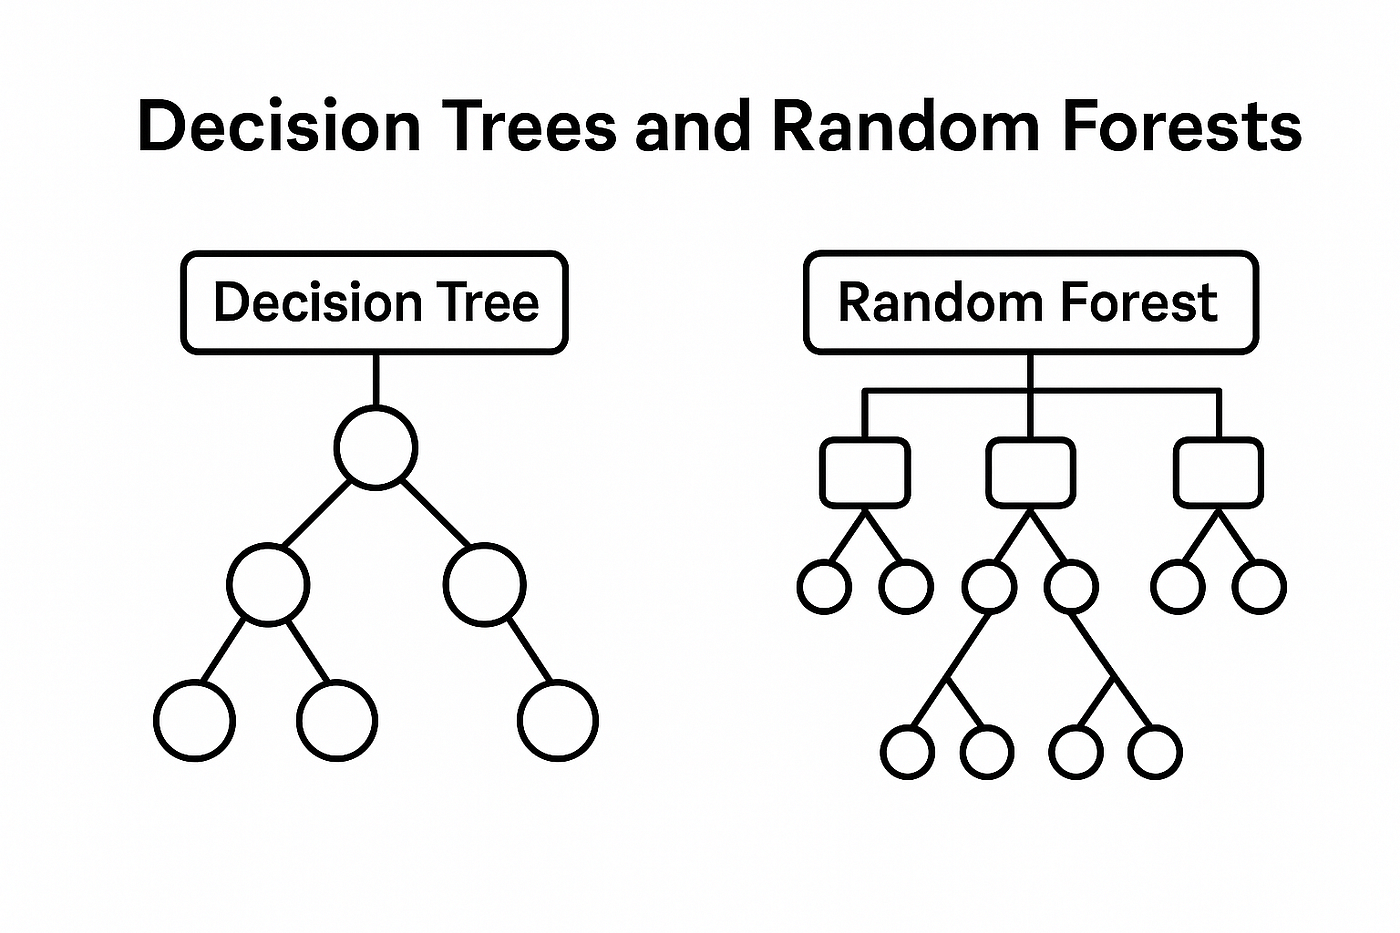
\includegraphics[width=0.5\linewidth]{IMAGE/random forest.png}
    \caption{Cây quyết định và rừng ngẫu nhiên.}
\end{figure}
\textbf{\large K}\textbf{hái niệm} 

Rừng ngẫu nhiên (\textit{Random Forest}) là một mô hình học có giám sát được phát triển nhằm giải quyết các bài toán phân lớp và hồi quy với hiệu suất vượt trội so với mô hình cây quyết định (\textit{Decision Tree}) đơn lẻ. Tương tự như một khu rừng được hình thành từ nhiều cây, mô hình này bao gồm một tập các cây quyết định được xây dựng độc lập, mỗi cây được huấn luyện trên một tập dữ liệu con được tạo ngẫu nhiên từ tập dữ liệu huấn luyện ban đầu. Các dự đoán từ từng cây thành phần sau đó được tổng hợp lại - thông qua cơ chế bỏ phiếu đa số trong bài toán phân lớp hoặc trung bình hóa trong bài toán hồi quy - để tạo ra kết quả cuối cùng. 


Đặc trưng ``ngẫu nhiên''  trong rừng ngẫu nhiên được thể hiện qua hai yếu tố chính, đóng vai trò cốt lõi trong việc tối ưu hóa hiệu suất mô hình:
\begin{itemize}
    \item \textbf{Ngẫu nhiên hóa tập dữ liệu huấn luyện:} Quá trình này được thực hiện thông qua kỹ thuật \textit{bootstrapping}, một phương pháp lấy mẫu có lặp lại từ tập dữ liệu huấn luyện ban đầu. Mỗi tập dữ liệu con được tạo ra ngẫu nhiên, cho phép một số điểm dữ liệu xuất hiện nhiều lần trong cùng một tập, trong khi các điểm khác có thể bị loại bỏ. Kỹ thuật này, thường được gọi là \textit{bagging (bootstrap aggregating)}, đảm bảo rằng mỗi cây quyết định trong rừng được huấn luyện trên một tập con khác nhau, từ đó tăng cường tính đa dạng và giảm thiểu \textit{biến thiên} trong dự đoán. Sự lặp lại của các điểm dữ liệu trong quá trình lấy mẫu giúp mô hình thích nghi với các mẫu đặc trưng, đồng thời hạn chế tác động của nhiễu dữ liệu, một yếu tố quan trọng trong việc cải thiện độ tổng quát hóa.
    \item \textbf{Ngẫu nhiên hóa tập con thuộc tính:} Trong quá trình phân chia các nút nội bộ (\textit{internal node}) của mỗi cây quyết định, chỉ một tập con ngẫu nhiên của các thuộc tính được xem xét thay vì toàn bộ tập thuộc tính. Số lượng thuộc tính trong tập con thường được đặt bằng căn bậc hai của tổng số thuộc tính ban đầu, một quy tắc được đề xuất bởi Breiman để cân bằng giữa tính đa dạng và hiệu quả tính toán. Chẳng hạn, nếu tập dữ liệu có 16 thuộc tính, chỉ khoảng 4 thuộc tính được chọn ngẫu nhiên tại mỗi nút để xác định ngưỡng phân chia. Phương pháp này không chỉ tăng cường tính độc lập giữa các cây mà còn giảm nguy cơ quá khớp bằng cách hạn chế sự phụ thuộc vào một tập thuộc tính cố định.
\end{itemize}
Sự kết hợp của hai yếu tố ngẫu nhiên hóa kể trên tạo nên một mô hình có khả năng học linh hoạt từ dữ liệu phức tạp, đồng thời duy trì độ ổn định và độ chính xác cao hơn so với một cây quyết định đơn lẻ. Tuy vậy, việc lựa chọn các tham số như số lượng cây trong rừng hoặc kích thước tập con thuộc tính cần được cân nhắc cẩn trọng, nhằm tránh làm gia tăng chi phí tính toán mà không mang lại cải thiện đáng kể về hiệu suất.

\textbf{\large R}\textbf{ừng ngẫu nhiên khắc phục nhược điểm của cây quyết định} 

Cây quyết định là một mô hình học có giám sát được sử dụng phổ biến trong lĩnh vực học máy nhờ tính dễ hiểu và khả năng biểu diễn trực quan các quy tắc phân loại. Tuy nhiên, mô hình này còn tồn tại một số hạn chế đáng kể, ảnh hưởng đến hiệu quả áp dụng trong các bài toán quy mô lớn hoặc đòi hỏi độ chính xác cao. Một trong những nhược điểm quan trọng nhất của cây quyết định là hiện tượng quá khớp, đặc biệt khi dữ liệu huấn luyện có nhiều biến động hoặc nhiễu. Cây quyết định thường có xu hướng ghi nhớ chi tiết các đặc điểm cụ thể của tập huấn
luyện, và do đó có thể dẫn đến mô hình phù hợp quá mức với dữ liệu đã thấy, nhưng lại không tổng quát tốt với các dữ liệu mới, chưa thấy.

Ngoài ra, cây quyết định cũng có thể bị thiên lệch nếu dữ liệu huấn luyện không đủ đa dạng hoặc có sự phân bố không đồng đều của các lớp. Điều này có thể dẫn đến việc cây quyết định chỉ học được các quy tắc phân chia mà không phản ánh đúng được sự phân bố của dữ liệu tổng thể.

Cuối cùng, cây quyết định có thể gặp phải vấn đề không ổn định, tức là thay đổi nhỏ trong dữ liệu huấn luyện có thể dẫn đến sự thay đổi lớn trong cấu trúc của cây. Điều này làm cho cây quyết định có thể trở nên khá nhạy cảm với những thay đổi trong tập huấn luyện và gây khó khăn trong việc xây dựng mô hình đáng tin cậy.

Để khắc phục những hạn chế trên, rừng ngẫu nhiên được đề xuất như một phương pháp tiên tiến, tận dụng sự kết hợp của nhiều cây quyết định để nâng cao hiệu suất và khả năng thích nghi. Mô hình này xây dựng một tập hợp các cây quyết định song song, mỗi cây được huấn luyện trên một tập dữ liệu con ngẫu nhiên, và kết quả cuối cùng được tổng hợp thông qua cơ chế bỏ phiếu đa số (\textit{majority voting}) cho phân lớp hoặc trung bình hóa cho hồi quy. Sự cải tiến này không chỉ giải quyết các nhược điểm của cây quyết định mà còn mở ra tiềm năng ứng dụng trong các bài toán quy mô lớn. Rừng ngẫu nhiên có thể giải quyết các vấn đề của cây quyết định bằng cách:
\begin{itemize}
    \item \textit{Giảm hiện tượng quá khớp:} Việc huấn luyện nhiều cây quyết định trên các mẫu dữ liệu khác nhau giúp rừng ngẫu nhiên giảm thiểu hiện tượng quá khớp. Mỗi cây được xây dựng dựa trên một tập con khác biệt của dữ liệu (thông qua quá trình \textit{bootstrapping}), do đó mô hình tổng thể ít bị ảnh hưởng bởi các điểm dữ liệu nhiễu hoặc ngoại lai.
    \item \textit{Tăng tính đa dạng và độ ổn định:} Bằng cách sử dụng nhiều cây quyết định được huấn luyện trên các tập dữ liệu và tập thuộc tính khác nhau, rừng ngẫu nhiên có khả năng học từ các khía cạnh khác nhau của dữ liệu. Điều này giúp tạo ra một mô hình ổn định hơn và ít nhạy cảm với các biến động nhỏ trong tập huấn luyện.
    \item \textit{Tối ưu hóa quá trình chọn thuộc tính:} Thay vì sử dụng toàn bộ tập thuộc tính tại mỗi nút phân chia, rừng ngẫu nhiên chỉ lựa chọn ngẫu nhiên một tập con các thuộc tính. Chiến lược này giúp giảm thiểu sự thiên lệch trong việc học và tăng khả năng tổng quát hóa của mô hình.
    \item \textit{Hiệu suất thực nghiệm cao:} Trong nhiều bài toán thực tế, rừng ngẫu nhiên đạt được hiệu suất rất cao và thường khó bị vượt qua. Nhờ cơ chế bỏ phiếu, các cây quyết định có hiệu suất thấp hoặc bị quá khớp sẽ có ảnh hưởng hạn chế đến kết quả cuối cùng, trong khi các cây mạnh được ưu tiên. Việc kết hợp nhiều cây chất lượng cao giúp cải thiện độ chính xác phân loại so với việc sử dụng một cây quyết định đơn lẻ.
\end{itemize}

\textbf{\large G}\textbf{iải thuật}

\setcounter{algocf}{1} % Thiết lập bắt đầu từ Algorithm 2 (nếu bạn muốn hiện số 3.2 thì tuỳ chỉnh ở file chính)

\begin{algorithm}[H]
\DontPrintSemicolon
\caption{\texttt{RandomForestTrain} - Huấn luyện mô hình Random Forest}

\Input{ Tập huấn luyện $(X, Y)$ gồm $N$ mẫu;\newline
        Số lượng cây $B$;\newline
        Số đặc trưng ngẫu nhiên tại mỗi node: $m$}
\Output{ Tập hợp các cây $\{f_1, f_2, \dots, f_B\}$}

Khởi tạo rừng rỗng: $\mathcal{F} \leftarrow \emptyset$;\;

\For{$b = 1$ \KwTo $B$}{
    Lấy mẫu bootstrap $(X_b, Y_b)$ từ $(X, Y)$ bằng cách chọn $N$ mẫu có hoàn lại;\;
    
    Huấn luyện cây $f_b$ trên $(X_b, Y_b)$ với:\;\\
    \nonl \Indp $\bullet$ Tại mỗi node: chọn ngẫu nhiên $m$ đặc trưng và chia theo đặc trưng tốt nhất\; \Indm
    
    Thêm $f_b$ vào rừng: $\mathcal{F} \leftarrow \mathcal{F} \cup \{f_b\}$;\;
}
\textbf{return} $\mathcal{F}$\;
\end{algorithm}
\begin{algorithm}[H]
\DontPrintSemicolon
\caption{\texttt{RandomForestPredict} - Dự đoán với mô hình Random Forest}

\Input{ Mẫu mới $x$;\newline
        Tập huấn luyện $(X, Y)$;\newline
        Số cây $B$, số đặc trưng ngẫu nhiên $m$}
\Output{ Dự đoán $\hat{y}$}

Huấn luyện mô hình: $\mathcal{F} \leftarrow \texttt{RandomForestTrain}(X, Y, B, m)$;\;

Lấy dự đoán từ từng cây: $\hat{y}_b \leftarrow f_b(x), \quad \forall f_b \in \mathcal{F}$;\;

\textbf{return} \textit{Biểu quyết đa số (classification)} hoặc \textit{trung bình (regression)} của $\{\hat{y}_1, \dots, \hat{y}_B\}$\;
\end{algorithm}




\textbf{\large C}\textbf{ông thức} 

Dự đoán cuối cùng ($\hat{y}$) được xác định bằng cách lấy biểu quyết đa số từ các cây thành phần ($f_b$):
\begin{equation}
\hat{y} = \arg\max_y \sum_{b=1}^{B} I(f_b(x) = y)
\end{equation}
Trong đó $I(\cdot)$ là hàm chỉ thị và $B$ là số lượng cây trong rừng.

\subsubsection{Support Vector Machine (SVM)}

\textbf{\large G}\textbf{iới thiệu}

Trong số các thuật toán học máy được sử dụng cho bài toán này, thuật toán \textit{Support Vector Machine(SVM)} nổi bật như một phương pháp mạnh mẽ và hiệu quả, đặc biệt trong các bài toán phân loại nhị phân như phân biệt nguồn nước an toàn và không an toàn. Thuật toán này hoạt động bằng cách tìm một siêu phẳng (\textit{hyperplane}) trong không gian đặc trưng để tách biệt hai lớp với khoảng cách biên (margin) lớn nhất, đảm bảo khả năng tổng quát hóa tốt ngay cả khi dữ liệu mẫu nước có sự chồng chéo hoặc nhiễu. Điểm mạnh của SVM nằm ở khả năng xử lý các tập dữ liệu có chiều cao, chẳng hạn như các chỉ số hóa lý đa dạng của nước, và khả năng sử dụng kỹ thuật kernel để xử lý các trường hợp dữ liệu không tách biệt tuyến tính. Hơn nữa, SVM hỗ trợ khả năng điều chỉnh tham số, chẳng hạn như tham số C để cân bằng giữa lỗi phân loại và tối ưu hóa biên, giúp mô hình thích nghi tốt với các đặc trưng phức tạp của dữ liệu đánh giá chất lượng nước.

\textbf{\large K}\textbf{hái niệm} 

Thuật toán SVM là một phương pháp \textit{học máy có giám sát} được sử dụng chủ yếu cho các bài toán phân loại nhị phân (\textit{binary classification}), dù cũng có thể mở rộng cho phân loại đa lớp hoặc hồi quy. SVM hoạt động bằng cách xây dựng một siêu phẳng (hyperplane), là một không gian con $n-1$ chiều trong không gian đặc trưng n chiều, nhằm tách biệt hai lớp dữ liệu một cách tối ưu. Trong không gian hai chiều, siêu phẳng này là một đường thẳng phân chia mặt phẳng thành hai vùng, mỗi vùng đại diện cho một lớp dữ liệu.

Tính tối ưu của siêu phẳng được xác định thông qua việc tối đa hóa khoảng cách biên (\textit{margin}), tức là khoảng cách từ siêu phẳng đến các vector hỗ trợ (\textit{support vectors}) - các điểm dữ liệu gần nhất của mỗi lớp. Khoảng cách này thường được tính dựa trên độ đo Euclidean trong không gian đặc trưng, và khoảng cách biên lớn hơn giúp mô hình tổng quát hóa tốt hơn, giảm nguy cơ quá khớp khi dự đoán trên dữ liệu mới. Trong quá trình huấn luyện, SVM sử dụng tập dữ liệu có nhãn để xác định siêu phẳng tối ưu bằng cách giải bài toán tối ưu hóa, đảm bảo sự phân tách rõ ràng giữa các lớp.

Khi dữ liệu không thể tách biệt tuyến tính trong không gian đặc trưng ban đầu, SVM áp dụng kỹ thuật kernel để ánh xạ dữ liệu vào một không gian chiều cao hơn, nơi các lớp có thể được tách biệt. Tham số C trong SVM được sử dụng để điều chỉnh mức độ khoan dung đối với lỗi phân loại, cân bằng giữa tối ưu hóa khoảng cách biên và độ chính xác trên tập huấn luyện, giúp xử lý dữ liệu có nhiễu.

\begin{figure}[H]
    \centering
    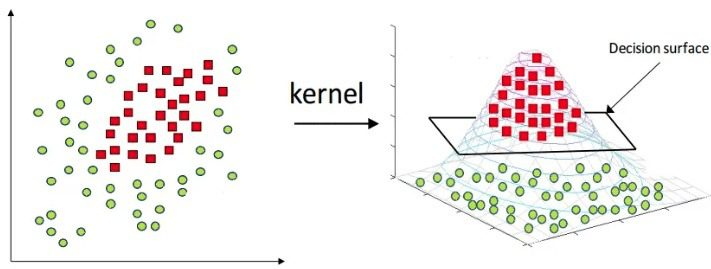
\includegraphics[width=0.5\linewidth]{IMAGE/kernel.jpg}
    \caption{Ánh xạ không gian đặc trưng bằng hàm kernel.}
\end{figure}
Sau khi huấn luyện, SVM phân loại dữ liệu mới bằng cách xác định vị trí của chúng trong không gian đặc trưng, dựa trên khoảng cách từ điểm dữ liệu đến siêu phẳng. Với khả năng xử lý các không gian đặc trưng cao chiều và dữ liệu phức tạp, SVM được ứng dụng rộng rãi trong các bài toán như nhận diện nguồn nước an toàn/không an toàn, phân loại văn bản, nhận diện hình ảnh, và phát hiện gian lận trong an ninh mạng.

\textbf{\large C}\textbf{ông thức và giải thuật}

%\textbf{1. Mô hình SVM cơ bản và Kí hiệu}

Trong bài toán phân loại nhị phân, tập dữ liệu huấn luyện bao gồm các cặp $(x^{(i)},y^{(i)})$, với $x^{(i)}\in\mathbb{R}^{n}$ là vector đặc trưng và nhãn lớp $y^{(i)}\in\{-1,1\}$. Việc sử dụng nhãn $\{-1,1\}$ giúp đơn giản hóa biểu diễn toán học của siêu phẳng phân chia $w^{T}x+b=0$. Bộ phân loại tuyến tính này được tham số hóa bởi vector trọng số $w\in\mathbb{R}^{n}$ và tham số chặn $b\in\mathbb{R}$. 

Hàm phân loại dự đoán được xác định như sau:
\begin{equation}
h_{w,b}(x)=\text{sign}(w^{T}x+b)
\end{equation}
Trong đó, $\text{sign}(z)=1$ nếu $z\ge0$ và $\text{sign}(z)=-1$ nếu $z<0$.

%\textbf{2. Hàm khoảng cách và Khoảng cách hình học}
Mục tiêu cốt lõi của giải thuật SVM là tìm một siêu phẳng tối ưu có khoảng cách biên (margin) lớn nhất. Khoảng cách này được tính từ siêu phẳng đến các vector hỗ trợ (support vectors) - là các điểm dữ liệu nằm gần nhất của mỗi lớp. 
\begin{itemize}
    \item Khoảng cách hình học (geometric margin) từ một điểm dữ liệu $x^{(i)}$ đến siêu phẳng được tính theo công thức: $\gamma^{(i)}=y^{(i)}\left(\left(\frac{w}{||w||_2}\right)^{T}x^{(i)}+\frac{b}{||w||_2}\right)$.
    \item Khoảng cách biên tổng giữa hai lớp là $\frac{2}{||w||}$. Để tối đa hóa khoảng cách biên này, giải thuật cần tối thiểu hóa đại lượng $||w||$, hay tương đương là tối thiểu hóa $\frac{1}{2}||w||^{2}$ để đảm bảo hàm mục tiêu là hàm lồi và dễ tính đạo hàm.
\end{itemize}
%\textbf{3. Bài toán tối ưu hóa dạng gốc (Primal Form)}

Giả sử tập dữ liệu có thể phân tách tuyến tính, bài toán tối ưu hóa tìm siêu phẳng phân chia của SVM được phát biểu dưới dạng:
\begin{equation}
\min_{w,b}\frac{1}{2}||w||^{2}
\end{equation}
Với điều kiện ràng buộc: $y^{(i)}(w^{T}x^{(i)}+b)\ge1$, với $i=1,2,...,m$.

Ràng buộc này đảm bảo mọi điểm dữ liệu đều được phân loại đúng và nằm ngoài hoặc nằm ngay trên lề (margin). Các điểm thỏa mãn đẳng thức $y^{(i)}(w^{T}x^{(i)}+b)=1$ chính là các vector hỗ trợ.
%\textbf{4. Bài toán đối ngẫu Lagrange (Dual Form)}

Khi số chiều đặc trưng $n$ lớn hoặc tập dữ liệu không thể phân tách tuyến tính, việc giải bài toán đối ngẫu mang lại hiệu quả cao hơn. Bằng cách áp dụng phương pháp nhân tử Lagrange, bài toán gốc được chuyển sang dạng đối ngẫu như sau:
\begin{equation}
\max_{\alpha}\sum_{i=1}^{m}\alpha_{i}-\frac{1}{2}\sum_{i,j=1}^{m}\alpha_{i}\alpha_{j}y^{(i)}y^{(j)}(x^{(i)})^{T}x^{(j)}
\end{equation}
Với các ràng buộc: 
\begin{itemize}
    \item $\alpha_{i}\ge0$, với $i=1,...,m$
    \item $\sum_{i=1}^{m}\alpha_{i}y^{(i)}=0$
\end{itemize}

Trong đó, $\alpha_i$ là các nhân tử Lagrange. Từ bài toán đối ngẫu, vector trọng số $w$ của siêu phẳng có thể được xác định lại thông qua công thức: $w=\sum_{i=1}^{m}\alpha_{i}y^{(i)}x^{(i)}$. Theo điều kiện Karush-Kuhn-Tucker (KKT), chỉ những vector hỗ trợ mới có $\alpha_i > 0$, do đó giải thuật chỉ cần dựa vào một số lượng nhỏ các vector hỗ trợ này để phân tách dữ liệu, giúp tiết kiệm bộ nhớ và tăng tốc độ tính toán.
% \textbf{5. Giải quyết dữ liệu phi tuyến với Hàm Kernel (Kernel Trick)}

Trong trường hợp dữ liệu không thể phân tách tuyến tính trong không gian ban đầu, SVM áp dụng kỹ thuật hàm kernel để ánh xạ dữ liệu vào một không gian đặc trưng nhiều chiều ($d$-chiều) nơi tồn tại siêu phẳng phân tách được hai lớp. 

Hàm mục tiêu đối ngẫu chỉ phụ thuộc vào tích vô hướng $(x^{(i)})^{T}x^{(j)}$, do đó có thể thay thế tích vô hướng này bằng hàm Kernel $K(x, z) = \phi(x)^T \phi(z)$ mà không cần tính toán trực tiếp ánh xạ đặc trưng $\phi(x)$. Một số hàm Kernel phổ biến được sử dụng bao gồm:
\begin{itemize}
    \item \textbf{Đa thức kernel (Polynomial kernel):} $K(x, z)=(x^{T}z+c)^{d}$
    \item \textbf{Gaussian kernel (hay RBF kernel):} $K(x, z)=\exp\left(-\frac{||x-z||^{2}}{2\sigma^{2}}\right)$
\end{itemize}
Mô hình tối ưu hóa hàm đối ngẫu Lagrange để xác định siêu phẳng phân cách:
\begin{equation}
L(\alpha) = \sum_{i=1}^{m} \alpha_i - \frac{1}{2} \sum_{i,j=1}^{m} \alpha_i \alpha_j y^{(i)} y^{(j)} K(x^{(i)}, x^{(j)})
\end{equation}
Trong đó, $\alpha_i$ là các nhân tử Lagrange và $K(x^{(i)}, x^{(j)})$ là hàm kernel giúp xử lý các mối quan hệ phi tuyến tính.

% \subsection{Mạng nơ-ron nhân tạo (Artificial Neural Network - ANN)}

% \textbf{\large G}\textbf{iới thiệu}

% Trong những thập kỷ gần đây, sự bùng nổ của dữ liệu lớn (Big Data) và sự tiến bộ vượt bậc của năng lực tính toán đã tạo điều kiện cho Mạng thần kinh nhân tạo (Artificial Neural Network - ANN) trở thành một trong những mô hình học máy mạnh mẽ và được ứng dụng rộng rãi nhất. Nằm trong nhánh Học sâu (Deep Learning), ANN đã chứng minh được sự ưu việt trong việc giải quyết các bài toán phức tạp mà các mô hình học máy truyền thống thường gặp khó khăn, chẳng hạn như nhận dạng hình ảnh, xử lý ngôn ngữ tự nhiên, phân tích chuỗi thời gian và các bài toán phân loại có tính phi tuyến tính cao. Sự linh hoạt và khả năng tự động học hỏi các biểu diễn đặc trưng (feature representations) từ dữ liệu thô đã đưa ANN trở thành nền tảng cho nhiều hệ thống trí tuệ nhân tạo hiện đại.

% \textbf{\large K}\textbf{hái niệm}

% Mạng thần kinh nhân tạo là một mô hình toán học và tính toán được thiết kế lấy cảm hứng từ cấu trúc và cơ chế hoạt động của mạng lưới hệ thần kinh sinh học trong não bộ con người. Cấu trúc cơ bản của một ANN bao gồm nhiều nút xử lý thông tin, được gọi là các nơ-ron nhân tạo (artificial neurons) hoặc perceptron, được tổ chức thành các lớp (layers) kết nối với nhau. Một kiến trúc ANN truyền thống (Feedforward Neural Network) thường bao gồm ba thành phần chính được minh họa trong Hình \ref{fig:ANN}:

% \begin{figure}[H]
%     \centering
%     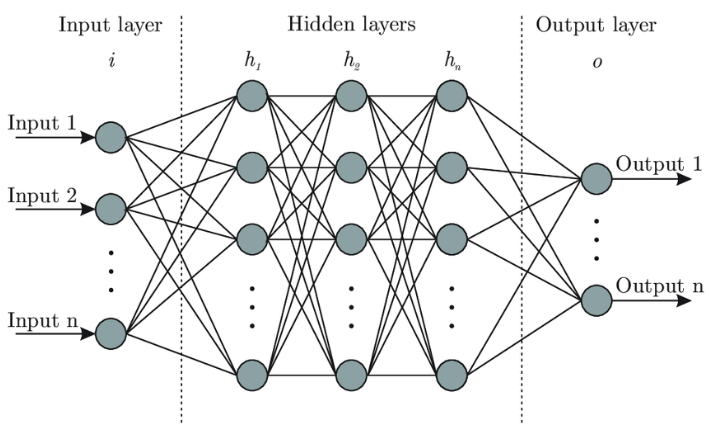
\includegraphics[width=0.5\linewidth]{IMAGE/ANN-1.png}
%     \caption{Mạng nơ-ron nhân tạo gồm lớp đầu vào, các lớp ẩn trung gian và lớp đầu ra.}
%     \label{fig:ANN}
% \end{figure}
% \begin{itemize}
%     \item \textbf{Lớp đầu vào (Input Layer):} Là nơi tiếp nhận dữ liệu ban đầu. Số lượng nơ-ron trong lớp này tương ứng với số lượng đặc trưng (features) của tập dữ liệu đầu vào.
%     \item \textbf{Các lớp ẩn (Hidden Layers):} Nằm giữa lớp đầu vào và lớp đầu ra, có nhiệm vụ trích xuất và học hỏi các quy luật, đặc trưng phi tuyến tính phức tạp ẩn sâu trong dữ liệu. Một mạng có thể có một hoặc nhiều lớp ẩn; số lượng lớp và số lượng nơ-ron trong mỗi lớp ảnh hưởng trực tiếp đến khả năng học (capacity) của mô hình.
%     \item \textbf{Lớp đầu ra (Output Layer):} Đưa ra kết quả dự đoán cuối cùng. Tùy thuộc vào loại bài toán, số lượng nơ-ron và hàm kích hoạt ở lớp này sẽ thay đổi (ví dụ: 1 nơ-ron với hàm Sigmoid cho bài toán phân loại nhị phân, hoặc nhiều nơ-ron với hàm Softmax cho bài toán phân loại đa lớp).
% \end{itemize}

% Thông tin trong ANN truyền thống chỉ di chuyển theo một hướng duy nhất: từ lớp đầu vào, qua các lớp ẩn, đến lớp đầu ra. Quá trình này được gọi là lan truyền tiến (Forward Propagation).

% \textbf{\large C}\textbf{ông thức tính toán tại mỗi nơ-ron}

% Tại mỗi nơ-ron trong các lớp ẩn và lớp đầu ra, dữ liệu đầu vào được xử lý thông qua hai phép toán cơ bản: tính tổng có trọng số (weighted sum) và áp dụng hàm kích hoạt (activation function).

% Giả sử một nơ-ron nhận $n$ tín hiệu đầu vào từ lớp trước đó, ký hiệu là $x_1, x_2, \dots, x_n$. Mỗi kết nối giữa các nơ-ron đều được gán một trọng số (weight) $w_i$, thể hiện mức độ quan trọng của tín hiệu đầu vào tương ứng. Ngoài ra, mỗi nơ-ron còn có một hệ số chệch (bias) $b$ giúp dịch chuyển đồ thị của hàm kích hoạt, tăng tính linh hoạt cho mô hình.

% Tổng có trọng số $z$ tại nơ-ron được tính bằng công thức:
% \begin{equation}
% z = \sum_{i=1}^{n} w_i x_i + b = \mathbf{w}^T \mathbf{x} + b
% \end{equation}

% Sau đó, giá trị $z$ này được truyền qua một hàm kích hoạt phi tuyến $f$ để tạo ra giá trị đầu ra $y$ của nơ-ron đó:
% \begin{equation}
% y = f(z) = f\left( \sum_{i=1}^{n} w_i x_i + b \right)
% \end{equation}

% Hàm kích hoạt đóng vai trò then chốt trong việc đưa tính phi tuyến vào mô hình, giúp ANN có khả năng học được các hàm phức tạp. Nếu không có hàm kích hoạt phi tuyến, một mạng ANN nhiều lớp cũng chỉ tương đương với một mô hình hồi quy tuyến tính đơn giản. Một số hàm kích hoạt phổ biến bao gồm:
% \begin{figure}[H]
%     \centering
    
%     % Đồ thị 1: ReLU
%     \begin{tikzpicture}
%         \begin{axis}[
%             width=5.5cm, height=5.5cm,
%             title={\textbf{ReLU}: $f(z) = \max(0, z)$},
%             axis lines=middle,
%             xmin=-5, xmax=5,
%             ymin=-1, ymax=5,
%             samples=100,
%             domain=-5:5,
%             grid=both,
%             grid style={line width=.1pt, draw=gray!30},
%             enlargelimits={abs=0.2}
%         ]
%         \addplot[blue, thick] {max(0, x)};
%         \end{axis}
%     \end{tikzpicture}
%     \hfill
%     % Đồ thị 2: Sigmoid
%     \begin{tikzpicture}
%         \begin{axis}[
%             width=5.5cm, height=5.5cm,
%             title={\textbf{Sigmoid}: $f(z) = \frac{1}{1 + e^{-z}}$},
%             axis lines=middle,
%             xmin=-5, xmax=5,
%             ymin=-0.2, ymax=1.2,
%             samples=100,
%             domain=-5:5,
%             grid=both,
%             grid style={line width=.1pt, draw=gray!30},
%             enlargelimits={abs=0.1}
%         ]
%         \addplot[red, thick] {1 / (1 + exp(-x))};
%         \end{axis}
%     \end{tikzpicture}
%     \hfill
%     % Đồ thị 3: Tanh
%     \begin{tikzpicture}
%         \begin{axis}[
%             width=5.5cm, height=5.5cm,
%             title={\textbf{Tanh}: $f(x) = \frac{e^z - e^{-z}}{e^z + e^{-z}}$},
%             axis lines=middle,
%             xmin=-5, xmax=5,
%             ymin=-1.2, ymax=1.2,
%             samples=100,
%             domain=-5:5,
%             grid=both,
%             grid style={line width=.1pt, draw=gray!30},
%             enlargelimits={abs=0.1}
%         ]
%         \addplot[green!60!black, thick] {tanh(x)};
%         \end{axis}
%     \end{tikzpicture}
    
%     \caption{Đồ thị các hàm kích hoạt phổ biến: ReLU, Sigmoid và Tanh.}
%     \label{fig:activation_functions}
% \end{figure}
% \begin{itemize}
%     \item \textbf{ReLU:} $f(z) = \max(0, z)$, phổ biến nhất trong các lớp ẩn vì tính toán nhanh và khắc phục được hiện tượng triệt tiêu đạo hàm (vanishing gradient).
%     \item \textbf{Sigmoid:} $f(z) = \frac{1}{1 + e^{-z}}$, nén giá trị đầu ra vào khoảng $(0, 1)$, thường dùng ở lớp đầu ra cho phân loại nhị phân.
%     \item \textbf{Tanh:} $f(z) = \frac{e^z - e^{-z}}{e^z + e^{-z}}$, nén giá trị vào khoảng $(-1, 1)$, thường hội tụ nhanh hơn Sigmoid.
% \end{itemize}

% \textbf{\large G}\textbf{iải thuật}

% Quá trình huấn luyện một mạng ANN thực chất là quá trình tối ưu hóa các tham số (trọng số $w$ và bias $b$) sao cho sai số giữa giá trị dự đoán của mạng và giá trị thực tế của dữ liệu huấn luyện là nhỏ nhất. Sai số này được đo lường bằng một Hàm mất mát (Loss Function), ví dụ như Mean Squared Error (MSE) cho bài toán hồi quy hoặc Binary Cross-Entropy (BCE) cho bài toán phân loại nhị phân.

% Giải thuật cốt lõi để huấn luyện ANN là \textbf{Lan truyền ngược (Backpropagation)} kết hợp với các thuật toán tối ưu hóa dựa trên \textbf{Đạo hàm giảm dần (Gradient Descent)}. Quy trình này diễn ra lặp đi lặp lại qua nhiều kỷ nguyên (epochs) với các bước chính như sau:

% \begin{enumerate}
%     \item \textbf{Lan truyền thuận (Forward Propagation):} Đưa một mẫu dữ liệu (hoặc một lô - batch dữ liệu) vào lớp đầu vào, tính toán qua các lớp ẩn để đưa ra kết quả dự đoán ở lớp đầu ra.
%     \item \textbf{Tính toán hàm mất mát (Compute Loss):} So sánh kết quả dự đoán với nhãn thực tế để tính toán giá trị của Hàm mất mát $L$.
%     \item \textbf{Lan truyền ngược (Backpropagation):} Bắt đầu từ lớp đầu ra, áp dụng quy tắc chuỗi (chain rule) trong vi tích phân để tính toán đạo hàm riêng (gradient) của Hàm mất mát theo từng trọng số và bias trong mạng: $\frac{\partial L}{\partial w_{ij}}$ và $\frac{\partial L}{\partial b_i}$. Gradient này cho biết mỗi tham số đóng góp bao nhiêu vào sai số tổng thể.
%     \item \textbf{Cập nhật trọng số (Weight Update):} Sử dụng thuật toán Gradient Descent (hoặc các biến thể cải tiến như Adam, RMSprop) để điều chỉnh các trọng số và bias theo hướng làm giảm hàm mất mát. Công thức cập nhật cơ bản là:
%     \begin{equation}
%     w_{ij} := w_{ij} - \eta \frac{\partial L}{\partial w_{ij}}
%     \end{equation}
%     \begin{equation}
%     b_i := b_i - \eta \frac{\partial L}{\partial b_i}
%     \end{equation}
%     Trong đó, $\eta$ là Tốc độ học (Learning rate), một siêu tham số quyết định bước nhảy của thuật toán trong không gian tối ưu.
% \end{enumerate}
% % ==========================================
% % 1. SƠ ĐỒ LAN TRUYỀN THUẬN (FORWARD PROPAGATION)
% % ==========================================
% \begin{figure}[H]
%     \centering
%     \begin{tikzpicture}[
%         scale=0.7, transform shape, % Thu nhỏ tỷ lệ xuống 0.7
%         input/.style={circle, draw=blue!70, thick, fill=blue!10, minimum size=1.2cm},
%         bias/.style={circle, draw=gray!70, thick, fill=gray!10, minimum size=1.2cm},
%         neuron/.style={circle split, draw=green!70!black, thick, fill=green!10, minimum size=3.5cm, align=center},
%         output/.style={circle, draw=orange!70, thick, fill=orange!10, minimum size=1.2cm},
%         loss/.style={rectangle, draw=red!70, thick, fill=red!10, minimum size=1.2cm, rounded corners},
%         arrow/.style={-Stealth, thick, draw=black!80},
%         label/.style={midway, fill=white, inner sep=2pt, font=\small}
%     ]

%         % Khai báo các Nút (Nodes)
%         \node[input] (x1) at (0, 3) {$x_1$};
%         \node[input] (x2) at (0, 1) {$x_2$};
%         \node (dots) at (0, -0.5) {$\vdots$};
%         \node[input] (xn) at (0, -2) {$x_n$};
%         \node[bias] (b)  at (0, 5) {$1$};

%         % Nơ-ron trung tâm (Chia làm 2 nửa: Tính tổng và Kích hoạt)
%         \node[neuron] (n) at (6, 1) {$z = \sum_{i=1}^n w_i x_i + b$ \nodepart{lower} $y = f(z)$};

%         % Output và Loss
%         \node[output] (y) at (10, 1) {$y$};
%         \node[loss] (L) at (13, 1) {$L(y, y_{true})$};

%         % Vẽ các mũi tên (Forward)
%         \draw[arrow] (x1) -- (n.160) node[label] {$w_1$};
%         \draw[arrow] (x2) -- (n.180) node[label] {$w_2$};
%         \draw[arrow] (xn) -- (n.200) node[label] {$w_n$};
%         \draw[arrow] (b)  -- (n.145) node[label] {$b$};

%         \draw[arrow] (n.0) -- (y) node[label] {};
%         \draw[arrow] (y) -- (L) node[label] {Tính Loss};

%     \end{tikzpicture}
%     \caption{Quá trình Lan truyền thuận (Forward Propagation) tại một Nơ-ron nhân tạo.}
%     \label{fig:forward_prop}
% \end{figure}

% % ==========================================
% % 2. SƠ ĐỒ LAN TRUYỀN NGƯỢC (BACKWARD PROPAGATION)
% % ==========================================
% \begin{figure}[H]
%     \centering
%     \begin{tikzpicture}[
%         scale=0.7, transform shape, % Thu nhỏ tỷ lệ xuống 0.7
%         input/.style={circle, draw=blue!70, thick, fill=blue!10, minimum size=1.2cm},
%         bias/.style={circle, draw=gray!70, thick, fill=gray!10, minimum size=1.2cm},
%         neuron/.style={circle split, draw=green!70!black, thick, fill=green!10, minimum size=3.5cm, align=center},
%         output/.style={circle, draw=orange!70, thick, fill=orange!10, minimum size=1.2cm},
%         loss/.style={rectangle, draw=red!70, thick, fill=red!10, minimum size=1.2cm, rounded corners},
%         backarrow/.style={Stealth-, thick, red, dashed},
%         label/.style={midway, fill=white, inner sep=2pt, font=\small, text=red}
%     ]

%         % Vị trí các Nút giống hệt bên trên
%         \node[input] (x1) at (0, 3) {$x_1$};
%         \node[input] (x2) at (0, 1) {$x_2$};
%         \node (dots) at (0, -0.5) {$\vdots$};
%         \node[input] (xn) at (0, -2) {$x_n$};
%         \node[bias] (b)  at (0, 5) {$1$};

%         % Nơ-ron lúc này hiển thị gradient của Z
%         \node[neuron] (n) at (6, 1) {$\frac{\partial L}{\partial z} = \frac{\partial L}{\partial y} \cdot f'(z)$ \nodepart{lower} $y = f(z)$};

%         \node[output] (y) at (10, 1) {$y$};
%         \node[loss] (L) at (13, 1) {$L$};

%         % Làm mờ các đường Forward để làm nền
%         \begin{scope}[gray!30, -Stealth, thick]
%             \draw (x1) -- (n.160);
%             \draw (x2) -- (n.180);
%             \draw (xn) -- (n.200);
%             \draw (b)  -- (n.145);
%             \draw (n.0) -- (y);
%             \draw (y) -- (L);
%         \end{scope}

%         % Vẽ các đường Backward truyền đạo hàm (Màu đỏ, nét đứt, hơi uốn cong để không đè vạch cũ)
%         \draw[backarrow] (n.150) to[bend right=15] node[label] {$\frac{\partial L}{\partial w_1} = \frac{\partial L}{\partial z}x_1$} (x1.0);
%         \draw[backarrow] (n.175) to[bend right=15] node[label] {$\frac{\partial L}{\partial w_2} = \frac{\partial L}{\partial z}x_2$} (x2.0);
%         \draw[backarrow] (n.195) to[bend left=15]  node[label] {$\frac{\partial L}{\partial w_n} = \frac{\partial L}{\partial z}x_n$} (xn.0);
%         \draw[backarrow] (n.135) to[bend right=15] node[label] {$\frac{\partial L}{\partial b} = \frac{\partial L}{\partial z}$} (b.0);

%         \draw[backarrow] (n.30)  to[bend right=20] node[label] {$\frac{\partial L}{\partial y}$} (y.150);
%         \draw[backarrow] (y.30)  to[bend right=20] node[label] {$\frac{\partial L}{\partial y} = \nabla_y L$} (L.150);

%     \end{tikzpicture}
%     \caption{Quá trình Lan truyền ngược (Backward Propagation) tính Gradient tại một Nơ-ron nhân tạo.}
%     \label{fig:backward_prop}
% \end{figure}

% Quá trình này được lặp lại cho đến khi Hàm mất mát đạt đến một giá trị đủ nhỏ hoặc mô hình không còn cải thiện thêm, đánh dấu việc ANN đã "học" được cách biểu diễn dữ liệu và sẵn sàng để đưa ra dự đoán trên dữ liệu mới.

\subsubsection{XGBoost (Extreme Gradient Boosting)}

\textbf{\large G}\textbf{iới thiệu}

Trong lĩnh vực học máy, đặc biệt là khi làm việc với dữ liệu dạng bảng (tabular data), XGBoost (Extreme Gradient Boosting) được công nhận là một trong những thuật toán mạnh mẽ và gặt hái được nhiều thành công nhất. Được phát triển ban đầu bởi Tianqi Chen, XGBoost nhanh chóng thống trị các cuộc thi khoa học dữ liệu (như Kaggle) nhờ khả năng mang lại độ chính xác vượt trội và tốc độ thực thi cực nhanh. Sự kết hợp hoàn hảo giữa kỹ thuật học tập hợp (Ensemble Learning), khả năng tính toán song song (Parallel Processing), và các cơ chế chống quá khớp (Overfitting) đã giúp XGBoost trở thành sự lựa chọn hàng đầu cho cả các bài toán hồi quy lẫn phân lớp phức tạp.

\textbf{\large K}\textbf{hái niệm}

XGBoost là một phiên bản cải tiến tối ưu hóa của thuật toán Gradient Boosting. Thuật toán này hoạt động dựa trên nguyên lý kết hợp nhiều "mô hình học yếu" (weak learners) – thường là các cây quyết định (Decision Trees) – để tạo thành một "mô hình học mạnh" (strong learner). Quá trình này diễn ra một cách tuần tự (sequential): mỗi cây quyết định mới được xây dựng sẽ tập trung vào việc sửa chữa những sai lầm (residual errors) mà các cây trước đó đã mắc phải.

Điểm khác biệt cốt lõi khiến XGBoost trở nên "Extreme" (cực độ) so với Gradient Boosting truyền thống bao gồm:
\begin{itemize}
    \item \textbf{Tối ưu hóa đạo hàm bậc hai:} Sử dụng khai triển Taylor bậc hai (tính cả Gradient và Hessian) để xấp xỉ hàm mất mát, giúp mô hình hội tụ nhanh và chính xác hơn.
    \item \textbf{Chính quy hóa (Regularization):} Tích hợp sẵn các thành phần L1 (Lasso) và L2 (Ridge) vào hàm mục tiêu để kiểm soát cấu trúc của cây, phạt nặng các cây quá phức tạp, từ đó ngăn chặn hiệu quả hiện tượng quá khớp.
    \item \textbf{Nhận thức sự thưa thớt (Sparsity Awareness):} Tự động học được hướng rẽ tối ưu cho các giá trị khuyết thiếu (missing values) mà không cần phải điền khuyết trước.
\end{itemize}


\textbf{\large C}\textbf{ông thức toán học}

Giả sử mô hình bao gồm $K$ cây quyết định, giá trị dự đoán cuối cùng cho một mẫu $x_i$ là tổng dự đoán của tất cả các cây:
\begin{equation}
\hat{y}_i = \sum_{k=1}^{K} f_k(x_i), \quad f_k \in \mathcal{F}
\end{equation}
Trong đó, $\mathcal{F}$ là không gian của tất cả các cây quyết định.

Tại bước lặp thứ $t$, thuật toán cần tìm một cây $f_t$ mới để thêm vào mô hình nhằm tối thiểu hóa hàm mục tiêu (Objective Function). Hàm mục tiêu của XGBoost bao gồm hai phần: Hàm mất mát $\mathcal{L}$ (đo lường độ lệch giữa thực tế và dự đoán) và Thành phần chính quy hóa $\Omega$ (đo lường độ phức tạp của cây):
\begin{equation}
\text{Obj}^{(t)} = \sum_{i=1}^{n} l\left(y_i, \hat{y}_i^{(t-1)} + f_t(x_i)\right) + \Omega(f_t)
\end{equation}

Sử dụng khai triển Taylor bậc hai để xấp xỉ hàm mất mát, hàm mục tiêu được viết lại thành:
\begin{equation}
\text{Obj}^{(t)} \approx \sum_{i=1}^{n} \left[ g_i f_t(x_i) + \frac{1}{2} h_i f_t^2(x_i) \right] + \Omega(f_t)
\end{equation}
Với $g_i = \partial_{\hat{y}^{(t-1)}} l(y_i, \hat{y}^{(t-1)})$ là đạo hàm bậc một (Gradient) và $h_i = \partial^2_{\hat{y}^{(t-1)}} l(y_i, \hat{y}^{(t-1)})$ là đạo hàm bậc hai (Hessian) của hàm mất mát.

Thành phần chính quy hóa $\Omega(f_t)$ được định nghĩa bằng số lượng nút lá $T$ và bình phương trọng số $w$ của các nút lá đó:
\begin{equation}
\Omega(f_t) = \gamma T + \frac{1}{2} \lambda \sum_{j=1}^{T} w_j^2
\end{equation}

Từ đó, trọng số tối ưu $w_j^*$ cho nút lá $j$ và giá trị tối ưu của hàm mục tiêu có thể tính được bằng công thức:
\begin{equation}
w_j^* = -\frac{\sum_{i \in I_j} g_i}{\sum_{i \in I_j} h_i + \lambda}
\end{equation}

\textbf{\large G}\textbf{iải thuật huấn luyện}

Quá trình huấn luyện XGBoost thực chất là quá trình xây dựng từng cây quyết định để tối ưu hóa hàm mục tiêu nói trên. Giải thuật diễn ra qua các bước:

\begin{enumerate}
    \item \textbf{Khởi tạo:} Bắt đầu với một giá trị dự đoán cơ sở $\hat{y}_i^{(0)}$ (thường là trung bình của nhãn hoặc 0.5 đối với phân loại nhị phân).
    \item \textbf{Lặp qua $t = 1$ đến $K$ (số lượng cây):}
    \begin{itemize}
        \item Tính toán giá trị Gradient ($g_i$) và Hessian ($h_i$) cho từng điểm dữ liệu dựa trên kết quả dự đoán của bước $t-1$.
        \item \textbf{Xây dựng cây $f_t$ (Thuật toán Exact Greedy hoặc Histogram-based):} Thuật toán duyệt qua các đặc trưng để tìm điểm chia (split) tốt nhất. Mức độ "tốt" của một điểm chia được đánh giá bằng độ lợi (Gain):
        \begin{equation}
        \text{Gain} = \frac{1}{2} \left[ \frac{G_L^2}{H_L + \lambda} + \frac{G_R^2}{H_R + \lambda} - \frac{(G_L + G_R)^2}{H_L + H_R + \lambda} \right] - \gamma
        \end{equation}
        Trong đó, $G_L, G_R, H_L, H_R$ lần lượt là tổng Gradient và Hessian của nhánh trái và nhánh phải. Nếu $\text{Gain} > 0$, thuật toán sẽ thực hiện tách nhánh.
        \item Gán trọng số $w_j^*$ cho các lá của cây $f_t$ vừa xây dựng.
    \end{itemize}
    \item \textbf{Cập nhật dự đoán:} Thêm cây mới vào quần thể kết hợp với hệ số học (Learning rate - $\eta$) để ngăn chặn cây học quá nhanh (Shrinkage):
    \begin{equation}
    \hat{y}_i^{(t)} = \hat{y}_i^{(t-1)} + \eta f_t(x_i)
    \end{equation}
    \item \textbf{Điều kiện dừng:} Quá trình lặp kết thúc khi đạt đủ số lượng cây $K$ hoặc kích hoạt cơ chế dừng sớm (Early Stopping) nếu hiệu suất trên tập kiểm thử không còn được cải thiện.
\end{enumerate}
